\documentclass[flalign]{article}
\usepackage[paper=a4paper,margin=1in]{geometry}
\usepackage{blindtext}
\usepackage{graphicx}
\usepackage{cite}
\usepackage{alphalph}

%\renewcommand\thesubsectiondis{\AlphAlph{\value{subsection}}.}% for the headings in the text
\renewcommand\thesubsection{\mbox{\thesection-\AlphAlph{\value{subsection}}}}% for the ToC, for example

\usepackage{fixltx2e}
\usepackage{amsmath}
\usepackage{amsfonts}
\usepackage{amssymb}
\usepackage{graphicx}
\usepackage{algorithm}
\usepackage{etoolbox}
\usepackage[noend]{algpseudocode}
\usepackage{fancyhdr}
\usepackage{setspace}
\usepackage{alltt}
\usepackage{color}
\usepackage{multirow}
\usepackage{float}
\makeatletter
\def\BState{\State\hskip-\ALG@thistlm}
\algrenewcommand\algorithmicindent{0.7em}%
\makeatother
%\newcommand{\subparagraph}{}


\begin{document}
	\title{Machine Learning with Large Datasets\\04-04-00-10-42-16-1-13300\\ Assignment 2}
	\date{November 11, 2017}
	\maketitle
	
	\begin{enumerate}
		\item	\textbf{Results:}
		\begin{table}[h]
			\centering
			\caption{Accuracies of In Multiclass Logistic Regression using Stochastic Gradient Descent in  \%}
			\begin{tabular}{|l|l|l|l|l|}
				\hline
				Train & Test  & Development \\ \hline
			 	98.7 & 91.8 & 90.9 \\ \hline
			\end{tabular}
		\end{table}
		\begin{table}[h]
			\centering
			\caption{Training Time And Testing Time in Seconds}
			\begin{tabular}{|l|l|l|l|}
				\hline
				Train & Test  \\ \hline
			 	30219 & 60 \\ \hline
			\end{tabular}
		\end{table}
		\begin{figure}[H]
			\centering
			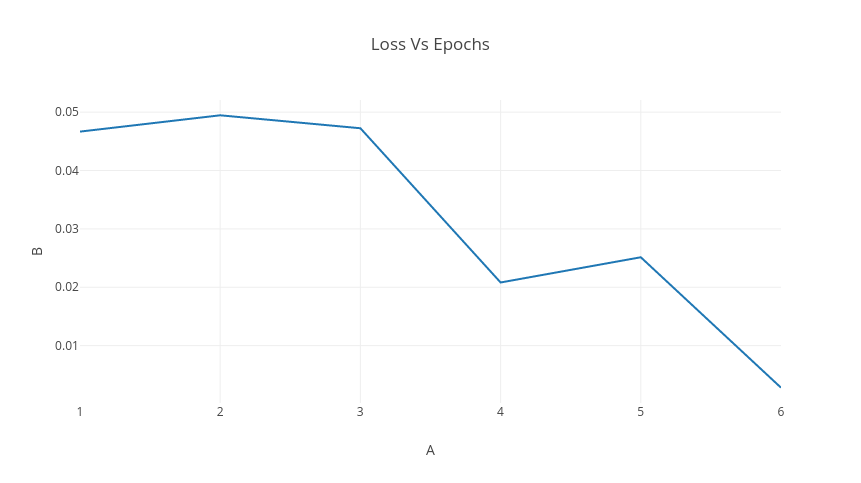
\includegraphics[scale=0.4]{f1.png}
			\caption{Plot of Loss vs Epoch}
		\end{figure}
		
		Reason For Numbers: Since the learning method is a stochastic approach, we are approximating the gradient by taking one row for its calculation. Hence the loss increased slightly first and then decreased. 
		
		\begin{table}[h]
			\centering
			\caption{Accuracies of In Multiclass Logistic Regression using Stochastic Gradient Descent in  \% with increasing learning rate}
			\begin{tabular}{|l|l|l|l|l|}
				\hline
				Train & Test  & Development \\ \hline
			 	98.7 & 83.3 & 82.7 \\ \hline
			\end{tabular}
		\end{table}
		\begin{table}[h]
			\centering
			\caption{Training Time And Testing Time in Seconds}
			\begin{tabular}{|l|l|l|l|}
				\hline
				Train & Test  \\ \hline
			 	18590 & 59 \\ \hline
			\end{tabular}
		\end{table}
		\begin{figure}[H]
			\centering
			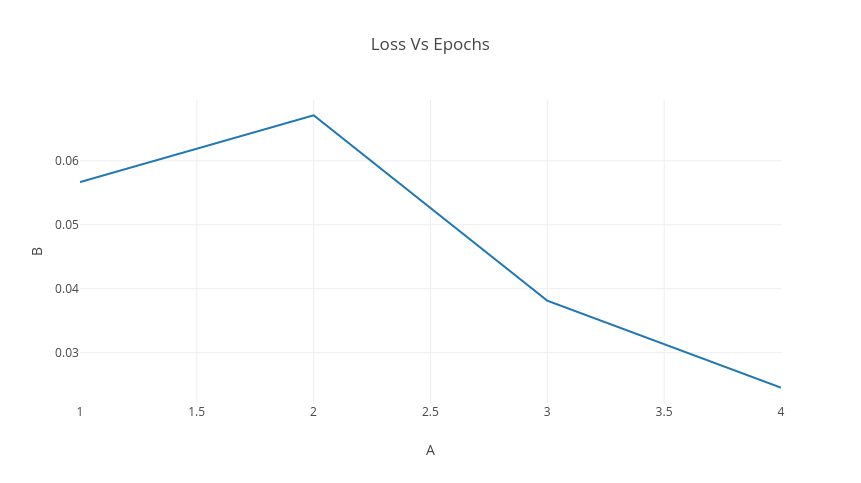
\includegraphics[scale=0.4]{f2.png}
			\caption{Plot of Loss vs Epoch}
		\end{figure}
		Reason For Numbers: Since the learning method is a stochastic approach, we are approximating the gradient by taking one row for its calculation. Hence the loss increased slightly first and then decreased. Since the learning rate is increasing, the rate of convergence is high because it is taking huge steps at a time. How ever, this huge steps means values can go high sometimes by skipping the minima. Hence the alternating increased in the graph
		\begin{table}[h]
			\centering
			\caption{Accuracies of In Multiclass Logistic Regression using Stochastic Gradient Descent in  \% with decreasing learning rate}
			\begin{tabular}{|l|l|l|l|l|}
				\hline
				Train & Test  & Development \\ \hline
			 	98.9 & 87.9 & 88.9 \\ \hline
			\end{tabular}
		\end{table}
		\begin{table}[h]
			\centering
			\caption{Training Time And Testing Time in Seconds}
			\begin{tabular}{|l|l|l|l|}
				\hline
				Train & Test  \\ \hline
			 	37289 & 59 \\ \hline
			\end{tabular}
		\end{table}
		\begin{figure}[H]
			\centering
			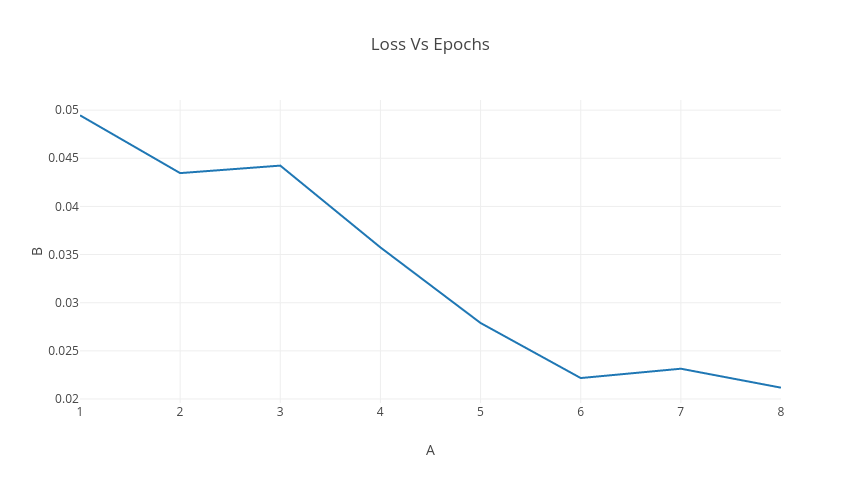
\includegraphics[scale=0.4]{f3.png}
			\caption{Plot of Loss vs Epoch}
		\end{figure}
		Reason For Numbers: Since the learning method is a stochastic approach, we are approximating the gradient by taking one row for its calculation. Hence the loss increased slightly first and then decreased. Since the learning rate is decreasing, the training will take longer time to converge as it is takes small steps to converge.
		\item The freezed hyperparameter alpha was 0.01 and lambda was 0.001 It is an API to be used in spark. For the second part, I have tried to implement the parameter server using DistML API.  I didnt get enough time to implement the parameter server since there was no support for the same API available in the internet.
I did run a Logistic regression on the spark machine once,using 1 parameter server, however it was holding all the resources and took around 8-9 hours to finish for training. It was an BSP implementation with maximum lag size of 2. I got a training accuracy of 96 \% and a test accuracy of 71 \%. I didn't get time to implement the rest.	
	\end{enumerate}

\end{document}